% Preamble - - - -
\documentclass[12pt]{article}
% Variables - - - -
\def\course{QSS 20}
\def\assignment{Literature Review}
\def\byline{Transit and The World Cup in the Greater Boston MSA}
\def\me{Roshan Karim}
\ifx\byline\empty
\def\subject{\course}
\else \def\subject{\course: \byline}
\fi
% - - - - Variables
% Commands - - - -
\newcommand{\opscale}[2]{\xrightarrow{#1r_#2 \text{→ } r_#2}}
\newcommand{\opreplace}[3]{\xrightarrow{r_#1 #2r_#3 \text{→ } r_#1}}
\newcommand{\opitc}[2]{\xrightarrow{r_#1 \text{↔} r_#2}}
% - - - - Commands
% Default Packages - - - -
\usepackage[letterpaper, total={6.5in, 9in}]{geometry}
\usepackage{fancyhdr}
\setlength{\headheight}{16pt}
\usepackage{titling}
\usepackage{citation-style-language}
\cslsetup{style = american-sociological-association}
\addbibresource{references.json}
\addbibresource{references.bib}
\usepackage{xurl}
\Urlmuskip=0mu plus 1mu
\setlength{\emergencystretch}{2em}
\usepackage[pdftitle={\assignment},
    pdfsubject={\subject},
    pdfauthor={\me},
    pdfproducer={LaTeX},
    pdfcreator={LuaLaTeX},
    colorlinks,
    citecolor=black,
urlcolor=blue]{hyperref}
\usepackage{graphicx}
\graphicspath{{./images/}}
\usepackage{parskip}
\usepackage[all]{nowidow}
% - - - - Default Packages
% Unique Packages - - - -
\usepackage{amsmath}
\usepackage{txfonts}
\usepackage{fontspec}
\setmainfont{Charis SIL}
\usepackage{bm}
\usepackage{tikz}
\usepackage{pgfplots}
\pgfplotsset{compat=newest}
% - - - - Unique Packages
% Header - - - -
\pagestyle{fancy}
\lhead{\course: \assignment}
\chead{\me}
\rhead{\today}
% - - - - Header
% - - - - Preamble
\begin{document}
% Title - - - -
\begingroup
\centering
\ifx\byline\empty
\LARGE\assignment\\
\else\LARGE\assignment\\\large\byline\\[1.5em]
\fi
\endgroup
% - - - - Title
% Content - - - -
\section{Introduction}
I began this literature review considering these three research questions:
\begin{enumerate}
    \item Are Greater Boston MSA neighborhoods with greater socioeconomic disadvantage disproportionately affected by unreliable transit?
    \item How does Greater Boston MSA transit accessibility shape access to employment opportunities?
    \item Do weather-related transit disruptions in the Greater Boston MSA disproportionately affect disadvantaged communities?
\end{enumerate}
I settle on a synthesis of these three research questions to better fit this course and contribute to the literature.
In the curated source list below, I place emphasis on the sources that best fit this synthesis.
\section{Curated Source List}
\subsection{Theory}
\begin{enumerate}
    \item \fullcite{martensTransportJusticeDesigning2017}
    \item \fullcite{lucasTransportSocialExclusion2012}
    \item \fullcite{pereiraDistributiveJusticeEquity2017}
\end{enumerate}
\subsection{Methodology}
\begin{enumerate}
    \item \fullcite{allenSizingTransportPoverty2019}
    \item \fullcite{draperDefinitionsRailwayPerformance2017}
    \item \fullcite{fuNewPerformanceIndex2007}
    \item \fullcite{lyuAnalyzingImpactService2026}
    \item \fullcite{welchMeasureEquityPublic2013}
\end{enumerate}
\subsection{Context-Specific Research}
\begin{enumerate}
    \item \fullcite{pereiraTransportLegacyMegaevents2018}
    \item \fullcite{pereiraTransportLegacyMegaevents2021}
\end{enumerate}
\subsection{Justification}
I selected sources that fit my research question, were well-cited and supported, and were largely peer-reviewed.
Beginning with theory, I chose \citet{martensTransportJusticeDesigning2017}, which is a foundational text linking sociology to transportation.
Concurrently, \citet{lucasTransportSocialExclusion2012} provides the evolution of transportation and social exclusion over history.
Finally, \citet{pereiraDistributiveJusticeEquity2017} contributes a qualitative perspective on the justice of transportation, which supports the relevance of my research question.

Second, I needed a robust selection of methodological resources to understand how best to conduct this research.
I looked to \citet{fuNewPerformanceIndex2007} for how to measure performance, \citet{welchMeasureEquityPublic2013} for how to measure equity, and \citet{lyuAnalyzingImpactService2026} for how to measure satisfaction.
\citet{draperDefinitionsRailwayPerformance2017} provides a comprehensive overview of existing railroad performance metrics for consideration, and \citet{allenSizingTransportPoverty2019} provides a battle-tested socioeconomic status measure perfect for transportation-related research.

Finally, I took advantage of context-specific research to understand the impact of the World Cup (as a proxy for large scale events and/or disasters) on transit equity.
\citet{pereiraTransportLegacyMegaevents2018} and \citet{pereiraTransportLegacyMegaevents2021} provide this valuable context.
\section{Mapping the Intersection of Sociology and Transportation}
\begin{center}
    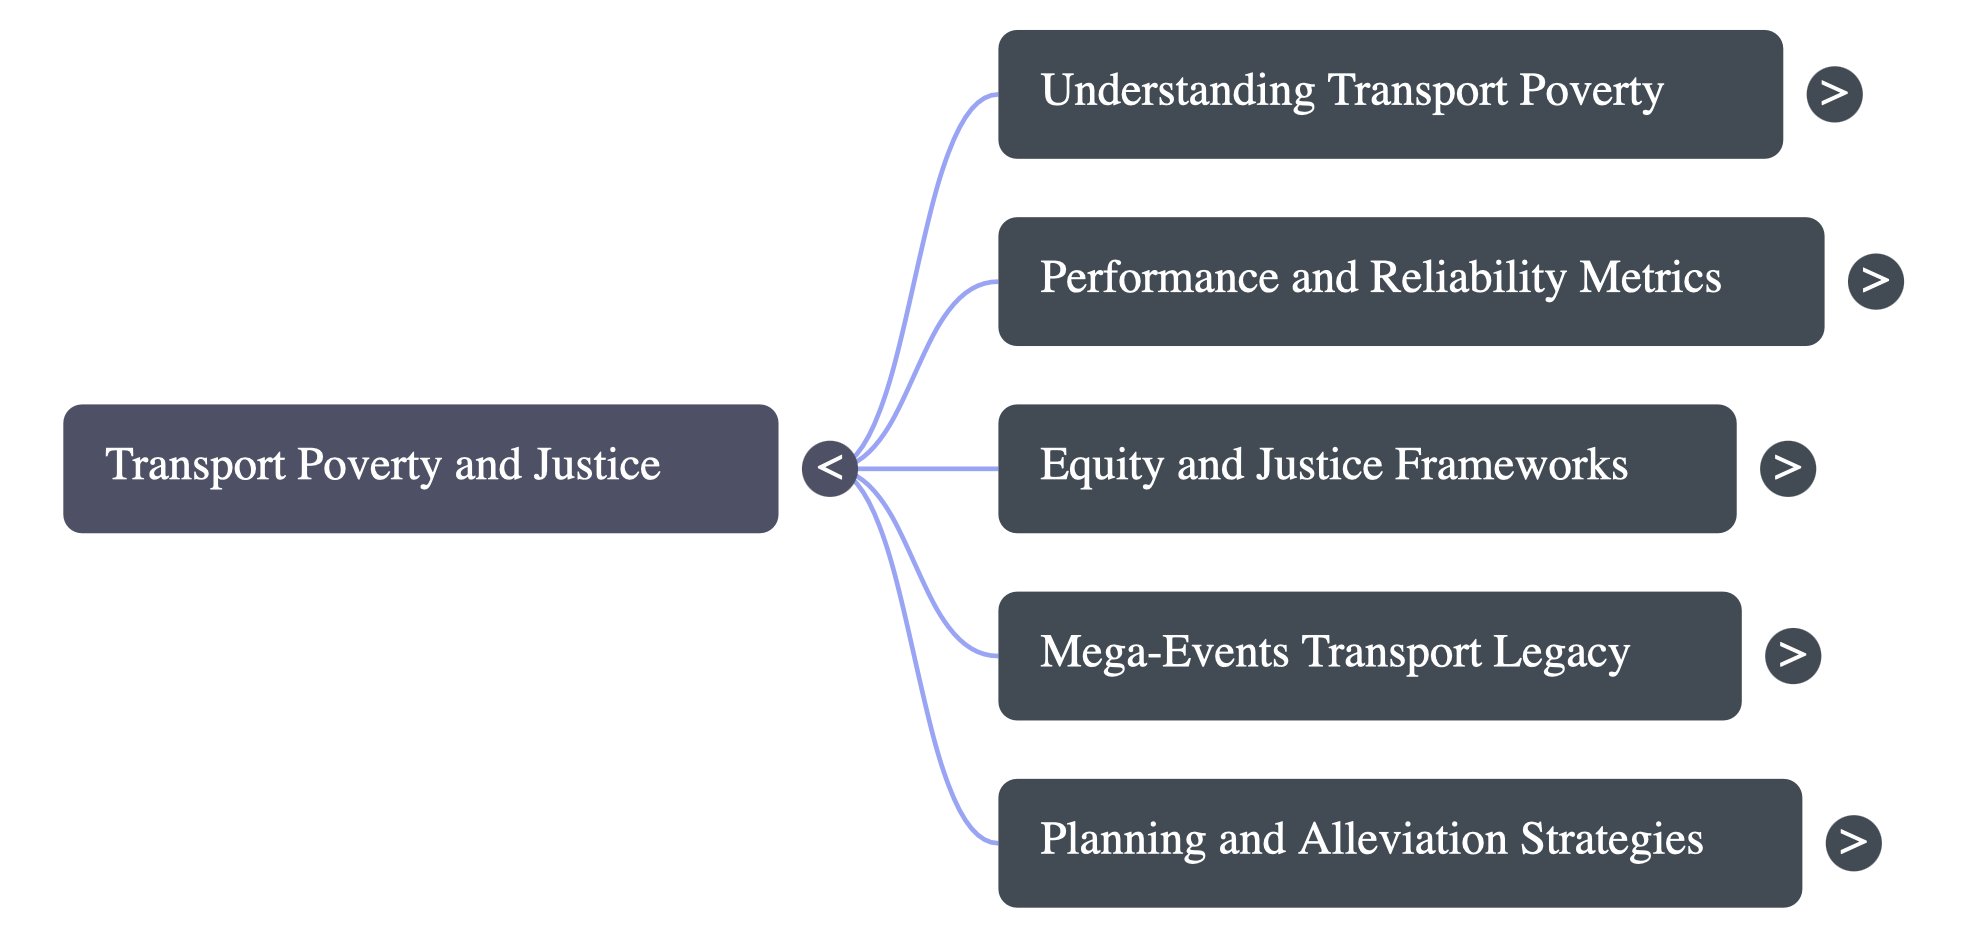
\includegraphics[width=0.5\textwidth]{images/mindmap.png}

    \small Figure 1: NotebookLM Mind Map
\end{center}
AAAAH

% - - - - Content
\end{document}